\documentclass{article}

\usepackage{graphicx}
\usepackage{tikz}
\usepackage{tikzsymbols}
\usetikzlibrary{calc,patterns,shapes.geometric}
\pagestyle{empty}
\usepackage[margin=0pt]{geometry}
\geometry{papersize={14in,12in}}

\def\centerarc[#1](#2)(#3:#4:#5){\draw[#1] ($(#2)+({#5*cos(#3)},{#5*sin(#3)})$) arc (#3:#4:#5);}

\begin{document}
	\begin{figure}
		\centering
		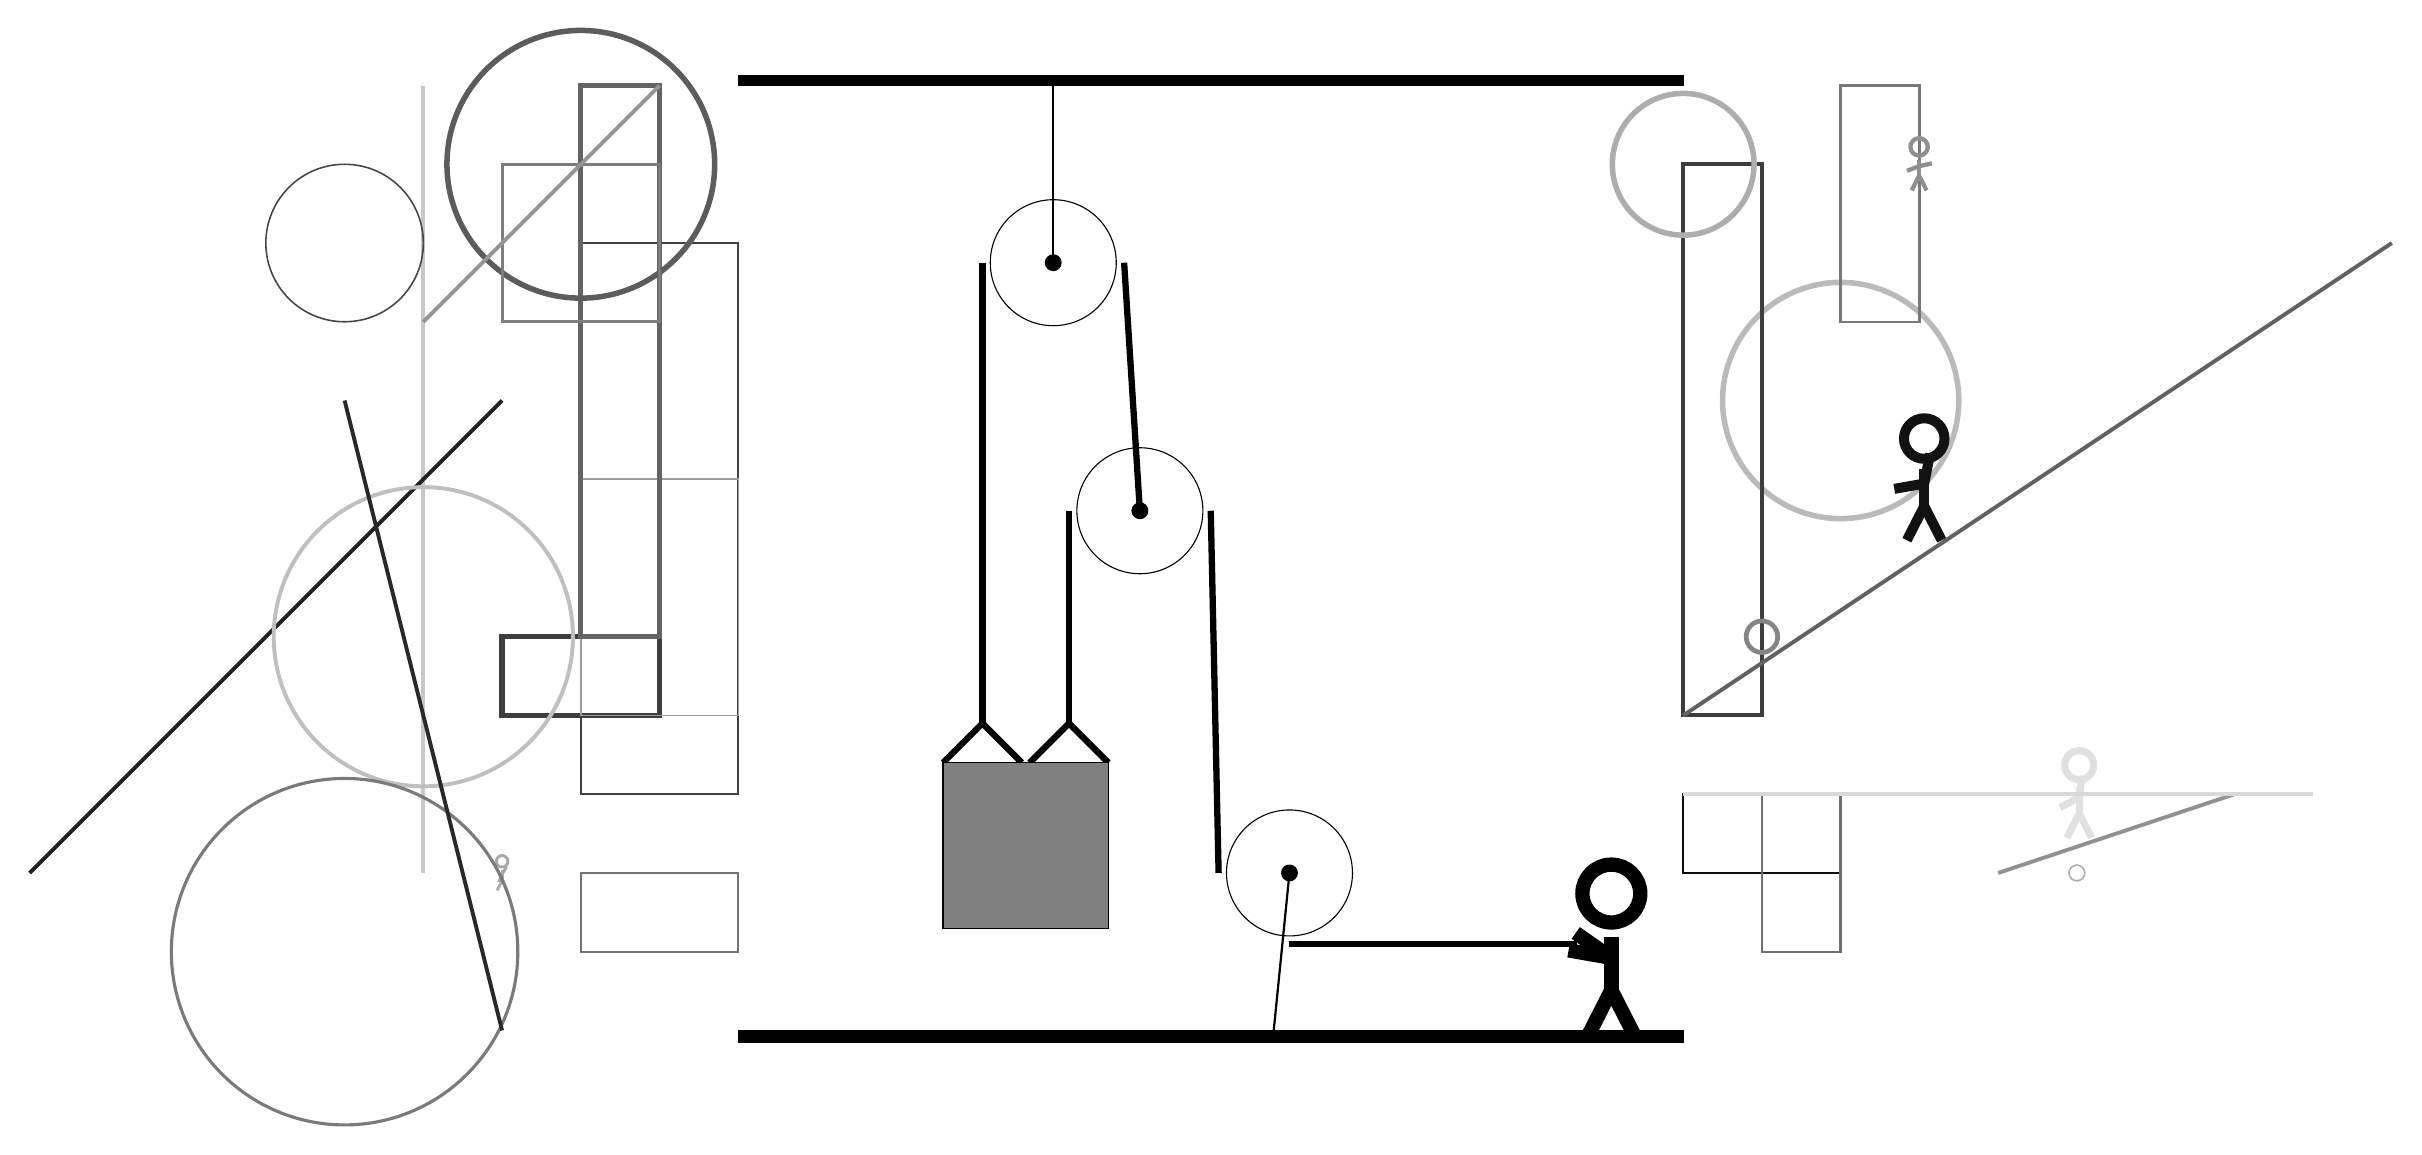
\begin{tikzpicture}
			%%%%% START %%%%%
			
			\draw[fill=black] (-2, 9) rectangle (10, 9.125);
			
			\draw (2, 6.75) circle (0.8);
			\draw[fill=black] (2, 6.75) circle (0.1);
			\draw[thick] (2, 6.75) -- (2, 9);
			
			\draw (3.1, 3.6) circle (0.8);
			\draw[fill=black] (3.1, 3.6) circle (0.1);
			
			\draw[line width=0.5mm, color=black!22](-6, 9) -- (-6, -1);
			
			\draw[line width=0.3mm, color=black!95] (12, -1) rectangle (10, 0);
			\draw [line width=0.7mm, color=black!27](12, 5) circle (1.5);
			\node[line width=0.2mm, color=black!34] at (-5, -1) {\Strichmaxerl[2][66][58]};
			\draw [line width=0.2mm, color=black!73](-7, 7) circle (1.0);
			
			\draw[line width=0.7mm, color=black!76] (-3, 2) rectangle (-5, 1);
			\draw [line width=0.2mm, color=black!33](15, -1) circle (0.1);
			\node[line width=0.2mm, color=black!93] at (13, 4) {\Strichmaxerl[7][10][79]};
			\draw[line width=0.3mm, color=black!75] (-4, 7) rectangle (-2, 0);
			\draw[line width=0.5mm, color=black!43](14, -1) -- (17, 0);
			\draw[line width=0.5mm, color=black!87](-5, 5) -- (-11, -1);
			
			\draw[line width=0.3mm, color=black!53] (12, 9) rectangle (13, 6);
			\node[line width=0.6mm, color=black!12] at (15, 0) {\Strichmaxerl[5][28][82]};
			\draw[line width=0.3mm, color=black!55] (-2, -1) rectangle (-4, -2);
			\draw[line width=0.3mm, color=black!56] (12, 0) rectangle (11, -2);
			\draw[line width=0.5mm, color=black!76] (10, 1) rectangle (11, 8);
			
			\node[line width=0.3mm, color=black!44] at (13, 8) {\Strichmaxerl[3][21][12]};
			\draw[line width=0.2mm, color=black!38] (-4, 1) rectangle (-2, 4);
			\draw [line width=0.6mm, color=black!48](11, 2) circle (0.2);
			
			\draw[line width=0.6mm, color=black!61] (-4, 9) rectangle (-3, 2);
			\draw [line width=0.7mm, color=black!32](10, 8) circle (0.9);
			\draw [line width=0.5mm, color=black!25](-6, 2) circle (1.9);
			\draw [line width=0.4mm, color=black!52](-7, -2) circle (2.2);
			\draw [line width=0.7mm, color=black!64](-4, 8) circle (1.7);
			\draw [line width=0.2mm, color=black!84](-6, 4) circle (0.0);
			
			\draw[line width=0.5mm, color=black!15](10, 0) -- (18, 0);
			\draw[line width=0.4mm, color=black!51] (-3, 8) rectangle (-5, 6);
			\draw[line width=0.5mm, color=black!61](10, 1) -- (19, 7);
			\draw[line width=0.5mm, color=black!42](-3, 9) -- (-6, 6);
			\draw[line width=0.5mm, color=black!84](-5, -3) -- (-7, 5);
			
			\draw (5, -1) circle (0.8);
			\draw[fill=black] (5, -1) circle (0.1);
			\draw[thick] (5, -1) -- (4.8, -3);
			
			\draw[line width = 0.8mm]  (0.6, 0.4) -- (1.1, 0.9) -- (1.6, 0.4);
			\draw[line width = 0.8mm]  (1.7, 0.4) -- (2.2, 0.9) -- (2.7, 0.4);
			\draw[fill=black!50] (0.6, 0.4) rectangle (2.7, -1.7);
			
			\draw[line width = 0.8mm] (1.1, 6.75) -- (1.1, 0.9);
			\centerarc[line width = 0.8mm](2, 6.75)(0:180:0.9);
			\draw[line width = 0.8mm] (2.9, 6.75) -- (3.1, 3.6);
			\draw[line width = 0.8mm] (2.2, 3.6) -- (2.2, 0.9);
			\centerarc[line width = 0.8mm](3.1, 3.6)(0:180:0.9);
			\draw[line width = 0.8mm] (4.0, 3.6) -- (4.1, -1);
			\centerarc[line width = 0.8mm](5, -1)(180:270:0.9);
			\draw[line width = 0.8mm] (5, -1.9) -- (8.65, -1.9);
			
			\node at (9, -2) {\Strichmaxerl[10][-35][170]};
			
			\draw[fill=black] (-2, -3) rectangle (10, -3.15);
			
			%%%%% END %%%%%
		\end{tikzpicture}
	\end{figure}	
\end{document}